\documentclass[11pt,a4paper]{article}
 
\usepackage[T1]{fontenc}
\usepackage[portuguese]{babel}
\usepackage{authblk}
\usepackage{listings}
\usepackage{enumitem}
\usepackage{graphicx}
\usepackage[hmargin=2cm,vmargin=3.5cm,bmargin=3cm]{geometry}
\usepackage[utf8]{inputenc}

\newcommand{\select}{\mbox{\Large$\sigma$}}

\pagenumbering{arabic}

\title{\textbf{Projecto de Bases de Dados, Parte 1}}
 
\author{Bruno Cardoso (72619), Lídia Freitas (78559) e Rodrigo Bernardo (78942)
} 

\affil{Instituto Superior T\'{e}cnico}

\begin{document}

\date{16 de Outubro de 2015}

\maketitle

\centerline{
\includegraphics[width=0.4\textwidth]{ist-simbolo.jpg}}

\begin{description}[noitemsep]
	\item \centering{Grupo 17}
	\item Turno: Quinta-Feira, ás 08h00, LAB 14
	\item 25 horas de trabalho por aluno.
\end{description}


\newpage

\tableofcontents
\newpage

\section{Modelo Entidade-Associa\c{c}\~ao}
\subsection{O Modelo}

\centerline{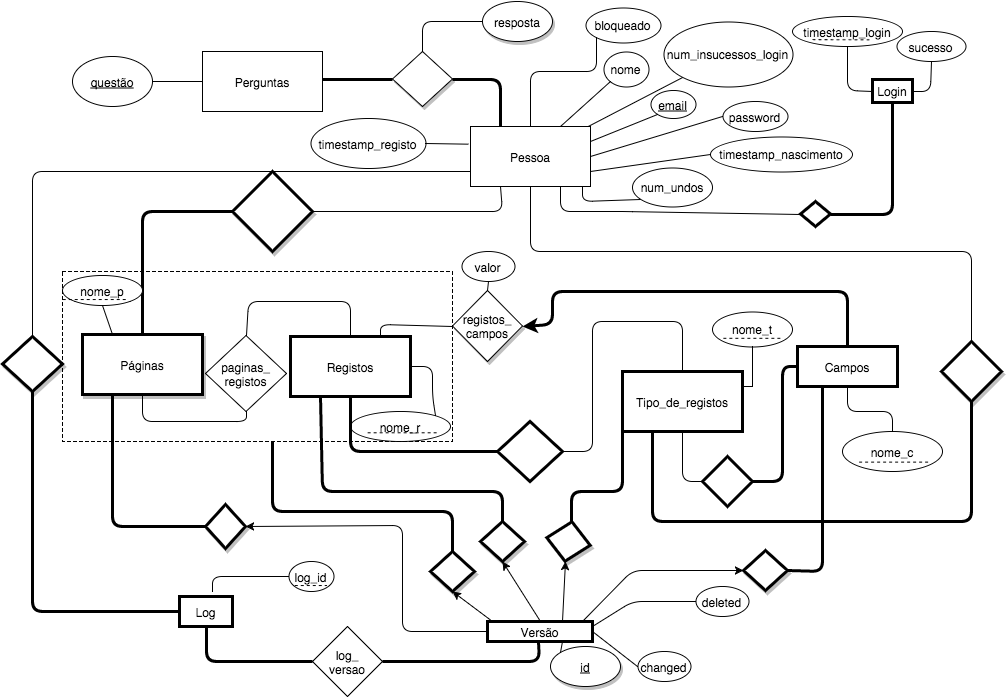
\includegraphics[width=1.0\textwidth]{modelo-ea-2.png}}

\newpage

\subsection{Restri\c{c}\~oes de Integridade do Modelo Entidade-Associa\c{c}\~ao}

\paragraph{}

O Modelo Entidade-Associação não limita todas as ocorrências possíveis e por isso podem dar-se situações fora do domínio do problema.

Como por exemplo, não se consegue assegurar que a ordem das datas estejam coerentes. Isto é, não é possível garantir que o timestamp\_nascimento seja inferior ao timestamp\_registo, ou que o timestamp\_login seja posterior ao timestamp\_registo.
Assim como não é possível assegurar que os números de tentativas de insucesso (num\_insucessos\_login) sejam positivos, ou o número de undo’s já realizados pela pessoa (num\_undos).
Outro aspecto que não é explicável através do modelo é o número de perguntas a que a pessoa responde, ou a unicidade da associação entre os objectos mutáveis (Páginas, páginas\_registos, Registos, Tipos\_de\_registos e Campos).
De forma a impedir que tais situações não ocorram, o Modelo Entidade-Associação é completado com as seguintes restrições de integridade:
\\

\begin{description}[itemsep=1.4em]
  \item[RI1] Na entidade \textit{Pessoa}, o atributo \textit{timestamp\_nascimento} \'{e} uma data anterior ao atributo \textit{timestamp\_registo}.
  \item[RI2] Na entidade \textit{Pessoa}, o atributo \textit{bloqueado} \'{e} um valor l\'{o}gico, verdadeiro ou falso.


  \item[RI3] Na entidade \textit{Pessoa}, o atributo \textit{num\_undos} \'{e} um n\'{u}mero inteiro positivo.


  \item[RI4] Na entidade \textit{Pessoa}, o atributo \textit{num\_insucessos\_login} \'{e} um n\'{u}mero inteiro positivo menor ou igual a 3.
  \item[RI5] Cada instância de \textit{Pessoa} associa-se, em cada instante, a duas instâncias da entidade \textit{Pergunta}.
  \item[RI6] Na entidade \textit{Login}, o atributo \textit{timestamp\_login} \'{e} uma data posterior ao atributo \textit{timestamp\_registo} de \textit{Pessoa}.
  \item[RI7] Na entidade \textit{Login}, o atributo \textit{sucesso} \'{e} um valor l\'{o}gico, verdadeiro ou falso.
  \item[RI8] Cada instância da entidade \textit{Versão} tem apenas uma associação activa a \textit{P\'{a}ginas}, \textit{paginas\_registos}, \textit{Registos}, \textit{Tipos\_de\_registos} e \textit{Campos}.
  \item[RI9] Na entidade \textit{Versão}, o atributo \textit{deleted} \'{e} um valor l\'{o}gico, verdadeiro ou falso.
  \item[RI10] Na entidade \textit{Versão}, o atributo \textit{changed} \'{e} um valor l\'{o}gico, verdadeiro ou falso.
  \item[RI11] Uma instância da entidade \textit{Versão} est\'{a} associada a uma ou duas instâncias da entidade \textit{Log}.
  \item[RI12] Uma instância da entidade \textit{Log} está associada a duas e s\'{o} duas instâncias da entidade \textit{Versão}.
  \item[RI13] Na entidade \textit{Log}, o atributo \textit{log\_id} \'{e} um inteiro positivo.
\end{description}

\newpage
\section{Modelo Relacional}
\subsection{O Modelo}

\begin{description}[noitemsep]
	\item\textit{ Pergunta(\underline{quest\~ao, email}, resposta)}
	\item\textit{ email: FK(Pessoa)}
	\item\textit{ notnull(resposta)}
\end{description}

\begin{description}[noitemsep]
	\item\textit{ Pessoa(\underline{email}, bloqueado, nome, num\_insucessos\_login, password, timestamp\_nascimento, timestamp\_registo, num\_undos)}
	\item\textit{ notnull(email)}
	\item\textit{ notnull(bloqueado)}
	\item\textit{ notnull(nome)}
	\item\textit{ notnull(num\_insucessos\_login)}
	\item\textit{ notnull(password)}
	\item\textit{ notnull(timestamp\_nascimento)}
	\item\textit{ notnull(timestamp\_registo)}
	\item\textit{ notnull(num\_undos)}
\end{description}

\begin{description}[noitemsep]
	\item\textit{ Login(\underline{timestamp\_login, email}, sucesso)}
	\item\textit{ email: FK(Pessoa)}
	\item\textit{ notnull(sucesso)}
\end{description}

\begin{description}[noitemsep]
	\item\textit{ P\'{a}ginas(\underline{nome\_p, email, id})}
	\item\textit{ email: FK(Pessoa)}
	\item\textit{ id: FK(Pessoa)}
\end{description}

\begin{description}[noitemsep]
	\item\textit{ P\'{a}ginas\_registos(\underline{nome\_p, email, nome\_r, nome\_t, id})}
	\item\textit{ nome\_p, email: FK(P\'{a}ginas)}
	\item\textit{ nome\_r, nome\_t, email: FK(Registos)}
	\item\textit{ id: FK(Vers\~{a}o)}
\end{description}

\begin{description}[noitemsep]
	\item\textit{ Registos(\underline{nome\_r, nome\_t, email, id})}
	\item\textit{ nome\_t, email: FK(tipos\_de\_registos)}
	\item\textit{ id: FK(Vers\~{a}o)}
\end{description}

\begin{description}[noitemsep]
	\item\textit{ Tipo\_de\_registos(\underline{nome\_t, email, id})}
	\item\textit{ email: FK(Pessoa)}
	\item\textit{ id: FK(Vers\~{a}o)}
\end{description}
\newpage

\begin{description}[noitemsep]
	\item\textit{ Campos(\underline{nome\_c, nome\_t, email, id})}
	\item\textit{ nome\_t, email: FK(Tipo\_de\_registos)}
	\item\textit{ id: FK(Vers\~{a}o)}
\end{description}

\begin{description}[noitemsep]
	\item\textit{ Registo\_Campos(\underline{nome\_r, nome\_t, nome\_c, email, id})}
	\item\textit{ nome\_r, nome\_t, email: FK(Registos)}
	\item\textit{ nome\_c, nome\_t, email: FK(Campos)}
	\item\textit{ id: FK(Vers\~{a}o)}
\end{description}


\begin{description}[noitemsep]
	\item\textit{ Vers\~{a}o(\underline{id}, changed, deleted)}
	\item\textit{ notnull(changed)}
	\item\textit{ notnull(deleted)}
\end{description}

\begin{description}[noitemsep]
	\item\textit{ Log(\underline{log\_id, email})}
	\item\textit{ email: FK(Pessoa)}
\end{description}

\begin{description}[noitemsep]
	\item\textit{ Log\_vers\~{a}o(\underline{log\_id, email, id})}
	\item\textit{ log\_id, email: FK(Log)}
	\item\textit{ id: FK(Vers\~{a}o)}
\end{description}

\newpage

\subsection{Restri\c{c}\~oes de Integridade do Modelo Relacional}

Ao passar do Modelo Entidade-Associa\c{c}\~{a}o para o Modelo Relacional \'{e} necess\'{a}rio
acrescentar restri\c{c}\~{o}es de integridade que antes n\~{a}o eram necess\'{a}rias. \`{A}s
restri\c{c}\~{o}es de dom\'{\i}nio j\'{a} indicadas, adicionam-se agora as restri\c{c}\~{o}es de
integridade referencial (sendo que de chave n\~{a}o temos nenhuma), as quais n\~{a}o
eram antes necess\'{a}rias considerar. Assim, as restri\c{c}\~{o}es RIn, com n \textgreater{} 13, s\~{a}o
restri\c{c}\~{o}es novas, exclusivas do Modelo Relacional, para cobrir casos que n\~{a}o s\~{a}o
poss\'{\i}veis modelar directamente neste modelo.

\begin{description}[itemsep=1.5em]
  \item[RI1] Na entidade \textit{Pessoa}, o atributo \textit{timestamp\_nascimento} \'{e} uma data anterior ao atributo \textit{timestamp\_registo}.
  \item[RI2] Na entidade \textit{Pessoa}, o atributo \textit{bloqueado} \'{e} um valor l\'{o}gico, verdadeiro ou falso.


  \item[RI3] Na entidade \textit{Pessoa}, o atributo \textit{num\_undos} \'{e} um n\'{u}mero inteiro positivo.


  \item[RI4] Na entidade \textit{Pessoa}, o atributo \textit{num\_insucessos\_login} \'{e} um n\'{u}mero inteiro positivo menor ou igual a 3.
  \item[RI5] Cada instância de \textit{Pessoa} associa-se, em cada instante, a duas instâncias da entidade \textit{Pergunta}.
  \item[RI6] Na entidade \textit{Login}, o atributo \textit{timestamp\_login} \'{e} uma data posterior ao atributo \textit{timestamp\_registo} de \textit{Pessoa}.
  \item[RI7] Na entidade \textit{Login}, o atributo \textit{sucesso} \'{e} um valor l\'{o}gico, verdadeiro ou falso.
  \item[RI8] Cada instância da entidade \textit{Versão} tem apenas uma associação activa a \textit{P\'{a}ginas}, \textit{paginas\_registos}, \textit{Registos}, \textit{Tipos\_de\_registos} e \textit{Campos}.
  \item[RI9] Na entidade \textit{Versão}, o atributo \textit{deleted} \'{e} um valor l\'{o}gico, verdadeiro ou falso.
  \item[RI10] Na entidade \textit{Versão}, o atributo \textit{changed} \'{e} um valor l\'{o}gico, verdadeiro ou falso.
  \item[RI11] Uma instância da entidade \textit{Versão} est\'{a} associada a uma ou duas instâncias da entidade \textit{Log}.
  \item[RI12] Uma instância da entidade \textit{Log} está associada a duas e s\'{o} duas instâncias da entidade \textit{Versão}.
  \item[RI13] Na entidade \textit{Log}, o atributo \textit{log\_id} \'{e} um inteiro positivo.
  \item[RI14] Quando se elimina um tuplo da tabela \textit{Pessoa}, devem ser eliminados os
tuplos com igual valor para o atributo \textit{email} nas tabelas \textit{Pergunta}, \textit{Paginas},
\textit{Tipos\_de\_registos}, \textit{Log} e \textit{Login}, caso existam.

  \item[RI15]Quando se elimina um tuplo da tabela \textit{Paginas}, devem ser eliminados os
tuplos com valores id\^{e}nticos para os atributos \textit{nome\_p} e \textit{email} da tabela \textit{Paginas\_registos}, caso existam.

  \item[RI16] Quando se elimina um tuplo da tabela \textit{Registos}, devem ser eliminados os
tuplos com valores id\^{e}nticos para os atributos \textit{nome\_r}, \textit{nome\_t} e \textit{email} das
tabelas \textit{Paginas\_registos} e \textit{Registo\_Campos}, caso existam.

  \item[RI17]Quando se elimina um tuplo da tabela \textit{Vers\~{a}o}, devem ser eliminados os
tuplos com igual valor para o atributo \textit{id} nas tabelas \textit{Paginas}, \textit{Paginas\_registos},
\textit{Registos}, \textit{Tipo\_de\_registos}, \textit{Campos}, \textit{Registo\_Campos} e \textit{Log\_versao}, caso existam.


  \item[RI18] Quando se elimina um tuplo da tabela \textit{Tipos\_de\_registos}, devem ser
eliminados os tuplos com valor id\^{e}ntico para os atributos \textit{nome\_t} e \textit{email} nas
tabelas \textit{Registos} e \textit{Campos}, caso existam.

  \item[RI19] Quando se elimina um tuplo da tabela \textit{Campos}, devem ser eliminados os
tuplos com valor id\^{e}ntico para os atributos \textit{nome\_c}, \textit{nome\_t} e \textit{email} nas tabelas
\textit{Registo\_Campos}.

  \item[RI20]Quando se elimina um tuplo da tabela \textit{Log}, devem ser eliminados os tuplos
com valor igual para os atributos \textit{log\_id} e \textit{email} na tabela \textit{Log\_versao}.
  
\end{description}


\newpage
\section{\'{A}lgebra Relacional}
\subsection{Pergunta 1}

$\Pi_{\textit{nome\_t}}(\sigma_{\textit{email = 'Manel@Notebook.pt'}}(\textit{Tipo\_de\_registos)})$

\subsection{Pergunta 2}

$\Pi_{\textit{email}}$ (\textit{Pessoa} $ \bowtie \select_{\textit{sucesso=falso}} (\textit{Login})$ )

\subsection{Pergunta 3}

$\Pi_{\textit{timestamp\_nascimento}}(\sigma_{\textit{nome\_p = 'facebook'} \wedge \textit{nome\_r = 'facebook'}} \textit{Pessoa} \bowtie 
\\\rho\textit{( P, Paginas)} \bowtie_{\textit{P.email = R.email}} \rho( \textit{R, Registos)}) $

\section{Linguagem SQL}

\subsection{Pergunta 1}
\begin{lstlisting}

SELECT DISTINCT nome_t
FROM Tipo_de_registos
WHERE email="Manel@notebook.pt";
\end{lstlisting}

\subsection{Pergunta 2}

\begin{lstlisting}
SELECT DISTINCT Pessoa.email 
FROM Pessoa, Login 
WHERE Pessoa.email = Login.email AND sucesso = false;
\end{lstlisting}

\subsection{Pergunta 3}

\begin{lstlisting}
SELECT timestamp_nascimento
FROM Pessoa, Paginas, Registos 
WHERE Pessoa.email = Registos.email 
AND Pessoa.email = Paginas.email 
AND Paginas.nome_p = "facebook" 
AND Registos.nome_r = "facebook";
\end{lstlisting}








\end{document}